\documentclass{minimal}

\usepackage{tikz,tikz-qtree}

\begin{document}

\pgfnewsubpicture{s}

\begin{pgfpicture}
\begin{pgfsubpicture}
\pgfnode{rectangle}{center}{A}{a}{\pgfusepath{stroke}}
\end{pgfsubpicture}
\pgfsavesubpicture{s}

\begin{pgfsubpicture}
{\pgftransformshift{\pgfpoint{30pt}{0pt}}
\pgfnode{rectangle}{center}{B}{b}{\pgfusepath{stroke}}}
\end{pgfsubpicture}
\pgfmergesubpicture{s}

\pgfrestoresubpicture{s}

{\pgftransformrotate{30}
\pgftransformscale{0.75}{0.75}
\pgfplacesubpicture
}

{\pgftransformshift{\pgfpoint{0pt}{-30pt}}
\pgfnode{rectangle}{center}{C}{c}{\pgfusepath{stroke}}}
{\pgftransformshift{\pgfpoint{30pt}{-30pt}}
\pgfnode{rectangle}{center}{D}{d}{\pgfusepath{stroke}}}

\pgfpathmoveto{\pgfpointanchor{a}{east}}
\pgfpathlineto{\pgfpointanchor{b}{west}}
\pgfusepath{stroke}

\pgfpathmoveto{\pgfpointanchor{a}{south}}
\pgfpathlineto{\pgfpointanchor{c}{north}}
\pgfusepath{stroke}

\pgfpathmoveto{\pgfpointanchor{b}{south}}
\pgfpathlineto{\pgfpointanchor{d}{north}}
\pgfusepath{stroke}

\pgfpathmoveto{\pgfpointanchor{c}{east}}
\pgfpathlineto{\pgfpointanchor{d}{west}}
\pgfusepath{stroke}

\end{pgfpicture}

\Tree [.S [.NP [.Adj colorless ] [.Adj green ] [.N ideas ] ] [.VP [.VP [.V sleep ] ] [.Adv furiously ] ] ]
\Tree [.X 
	a a a a a a a a a a
	a a a a a a a a a a
	a a a a a a a a a a
	a a a a a a a a a a
	a a a a a a a a a a 
	]
	
\Tree 
  [.a [.a [.a [.a [.a [.a [.a [.a [.a [.a
  ] ] ] ] ] ] ] ] ] ]
  
  
  
\section{Testing tikz trees compatibility}

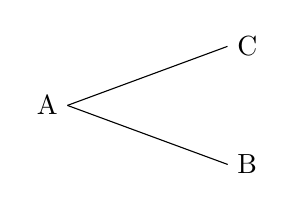
\begin{tikzpicture}[grow=right,level distance=1in]
\node {A} child {node {B}} child {node {C}};
\end{tikzpicture}
\begin{tikzpicture}[grow'=right,sibling distance=1in]
\node {A} child {node {B}} child {node {C}};
\end{tikzpicture}

  

\end{document}
